\chapter{Results}\label{cap:results}

\section{Baseline network activity}\label{sec:res_baseline}

Before the effects of neurogenesis were analyzed, it was first verified that the network settles into a stable and biologically
plausible behavior. Figure~\ref{fig:results-1}a shows the spiking activity of the EC, iGC, mGC and pCA3 populations during a
representative simulation. Driven by the EC input, the mGCs fire sparsely and in short, synchronized bouts, with only a small
fraction of the population active at any moment. The iGCs are more active, while the pCA3 cells fire at a moderate rate, spread
more evenly across the population.

This difference between the two populations can be seen in Figure~\ref{fig:results-1}b: the iGC firing-rate distribution is
shifted toward higher rates than that of the mGCs, with a median firing rate of \SI{3}{\hertz} against \SI{1}{\hertz} for the
mGCs. These values closely match those found \textit{in vivo} by~\textcite{mchughAdultborn2022} (\SI{2.3}{\hertz} for adult-born
against \SI{1.0}{\hertz} for mGCs), although the shape of the distribution differs. For every cell type, the model's firing rates
and population sparsity fell within the ranges compiled from the literature (Table~\ref{tab:firing_rates}), which is taken as
evidence that the network behaves plausibly.

\begin{figure}
    \centering
    \caption{Baseline network activity. \textbf{(a)} Raster plot of the spike times of the EC, iGC, mGC and pCA3 populations in a
        representative simulation, over the \SIrange{300}{1300}{\milli\second} recording window (the first \SI{300}{\milli\second}
        discarded for stabilization). \textbf{(b)} Kernel-density estimate of the per-cell firing-rate distribution in logarithmic
        scale of the mGC and iGC populations; the dashed lines mark the population medians (mGC, \SI{1}{\hertz}; iGC,
        \SI{3}{\hertz}).}

    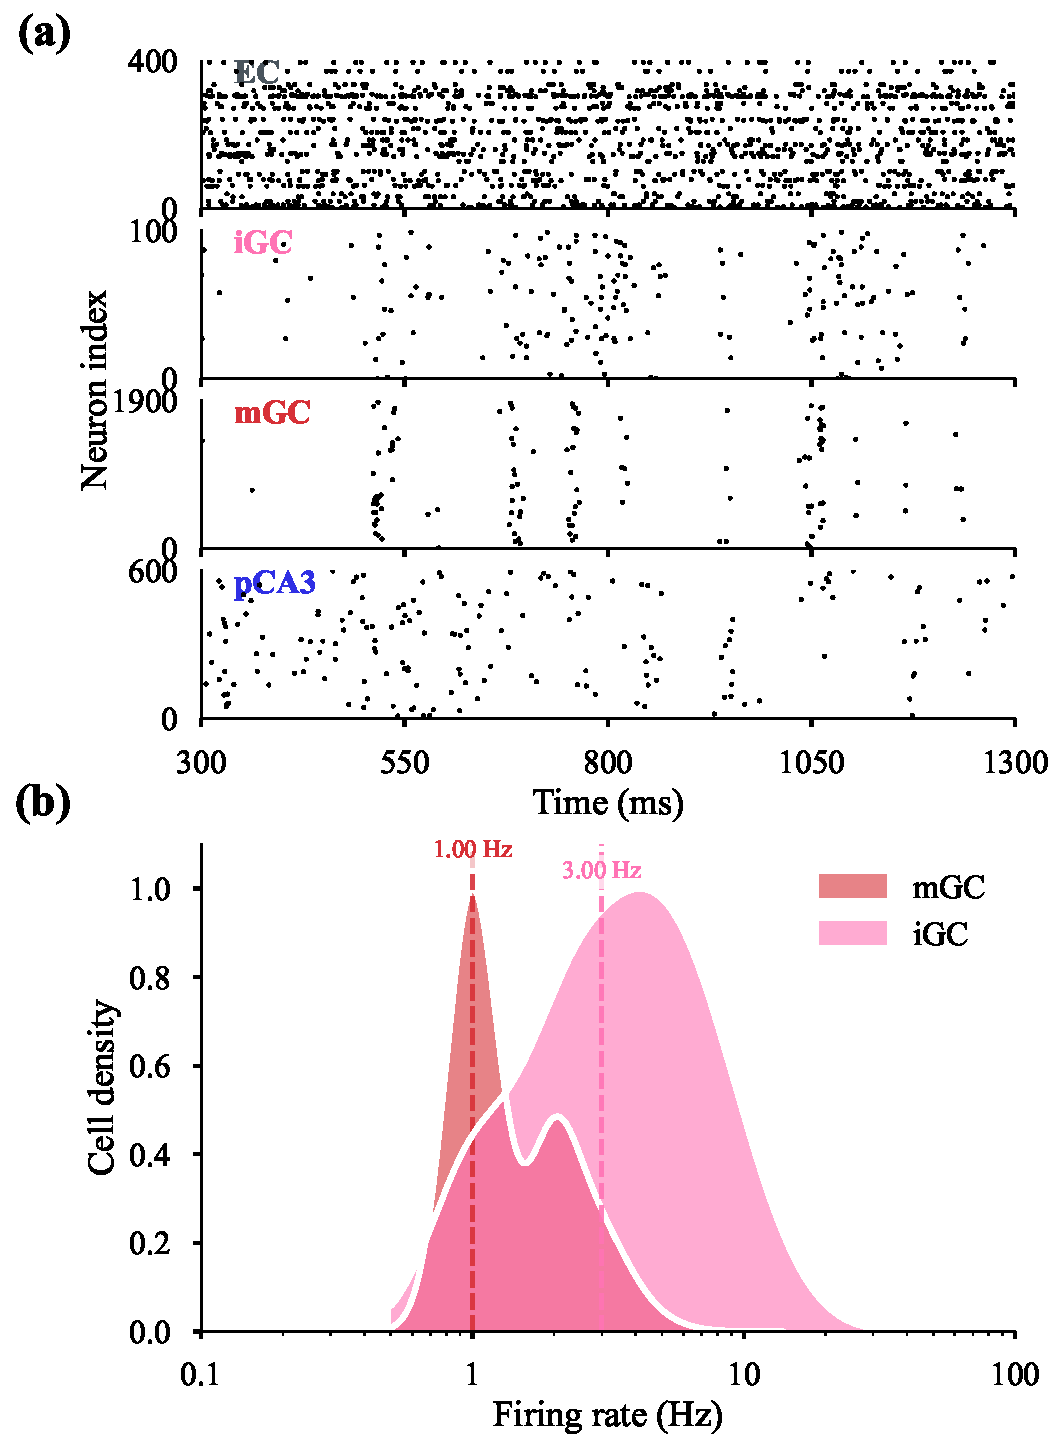
\includegraphics[width=0.85\textwidth]{figures/plots/baseline_panel.pdf}%
\label{fig:results-1}
\end{figure}

\section{Adult neurogenesis enhances pattern separation in the DG and CA3}\label{sec:res_separation}

Figure~\ref{fig:results-2}a shows that, with neurogenesis, the mGC population activation drops, and with each increase of the
EC$\to$iGC connection probability the mGC activation decreases further, from 7.9\% in the control network to 3.6\% at the highest
connection probability; the opposite is true for the iGC population, since a higher connection probability is expected to make the
iGCs more active, with almost 90\% of the iGC population being active for the highest connection probability simulated. This
happens because of the feedforward inhibition exerted by iGCs upon mGCs, via iGC $\to$ mGC, iGC $\to$ BC/HIPP $\to$ mGC and iGC
$\to$ MC $\to$ BC/HIPP $\to$ mGC\@. For increasing EC$\to$iGC connection probabilities, as mGC activity decreases and iGC activity
increases, an equilibrium of approximately 8\% of the entire GC population (iGCs and mGCs counted together) stays active,
similarly to the control model without neurogenesis.

This lower activation seen in the mGC population with adult neurogenesis directly affects pattern separation: with fewer neurons
active for a given pattern, the sparser coding leads to an increase in the mGC pattern separation degree, which rose monotonically
with the EC$\to$iGC connection probability from $\mathcal{S}_D = 2.40$ in the control network to $5.80$ at the full connection
probability (Spearman $\rho = 1.00$, $p < 10^{-6}$; Figure~\ref{fig:results-2}b). Resolved by input similarity, the mGC separation
showed the same ordering at every level, being strongest for the most similar inputs and higher than the control across the whole
similarity range (Figure~\ref{fig:pattern_separation_similarity}). The two GC types, however, behave in opposite ways. Taken on
their own, the iGC outputs never separate their inputs ($\mathcal{S}_D < 1$, falling from $0.45$ to $0.20$ as the connection
probability rises), acting instead as pattern integrators, as also reported by~\textcite{kimEffect2024}. When the whole GC
population is considered together, pattern separation remains above one but decreases with the EC$\to$iGC connection probability
(from $\mathcal{S}_D = 2.40$ to $1.22$; $\rho = -0.96$, $p < 10^{-5}$). Because the total GC activation stays near 8\% across
connection probabilities, this decline is driven almost entirely by a loss of output decorrelation, the mean pairwise correlation
between output patterns rising from $0.14$ to $0.55$, rather than by any change in activation. Since the role of iGCs is thought
to be the modulation of network activity rather than the encoding of information~\parencite{mchughAdultborn2022,
folszAdultborn2023}, the relevant quantity is the separation achieved by the encoding population, the mGCs, which is enhanced by
neurogenesis.

The same analysis applied to the pCA3 population (Figures~\ref{fig:results-2}c and~\ref{fig:results-2}d) shows that its mean
activation also decreases with neurogenesis and the EC$\to$iGC connection probability, from 29.7\% to 24.1\%, while its separation
degree increases in the same direction as that of the mGCs, from $\mathcal{S}_D = 0.51$ to $0.69$ ($\rho = +0.98$, $p < 10^{-5}$).
Unlike the DG, however, the pCA3 separation degree remains below one throughout: by the definition described in
Equation~\ref{eq:sd}, the CA3 keeps its outputs more alike than its inputs. This is expected of a region whose recurrent
connectivity supports autoassociation and pattern completion~\parencite{rollsMechanisms2013, kopsickFormation2024} rather than
separation. Neurogenesis therefore does not turn the CA3 into a separator, but pushes it toward separation.

\begin{figure}
    \centering
    \caption{Effects of adult neurogenesis and the EC$\to$iGC connection probability on activation, pattern separation and
        sparsity in the DG and CA3. In every panel the horizontal axis is the EC$\to$iGC connection probability (10--100\% of
        the EC$\to$mGC value), each point is the mean over the 30 pattern sets, shaded bands show the SEM and the dashed black
        line marks the control network without neurogenesis.
        \textbf{(a)} Mean population activation of DG GCs\@. \textbf{(b)} Pattern separation degree $\mathcal{S}_D$ of DG GCs; the
        gray dashed line marks $\mathcal{S}_D = 1$, above which the output patterns are more distinct than their inputs.
        \textbf{(c)} Mean population activation of the pCA3 cells. \textbf{(d)} Pattern separation degree of the pCA3 cells.
        \textbf{(e)} Population sparsity (Gini index) of the DG GCs and pCA3 cells.}

    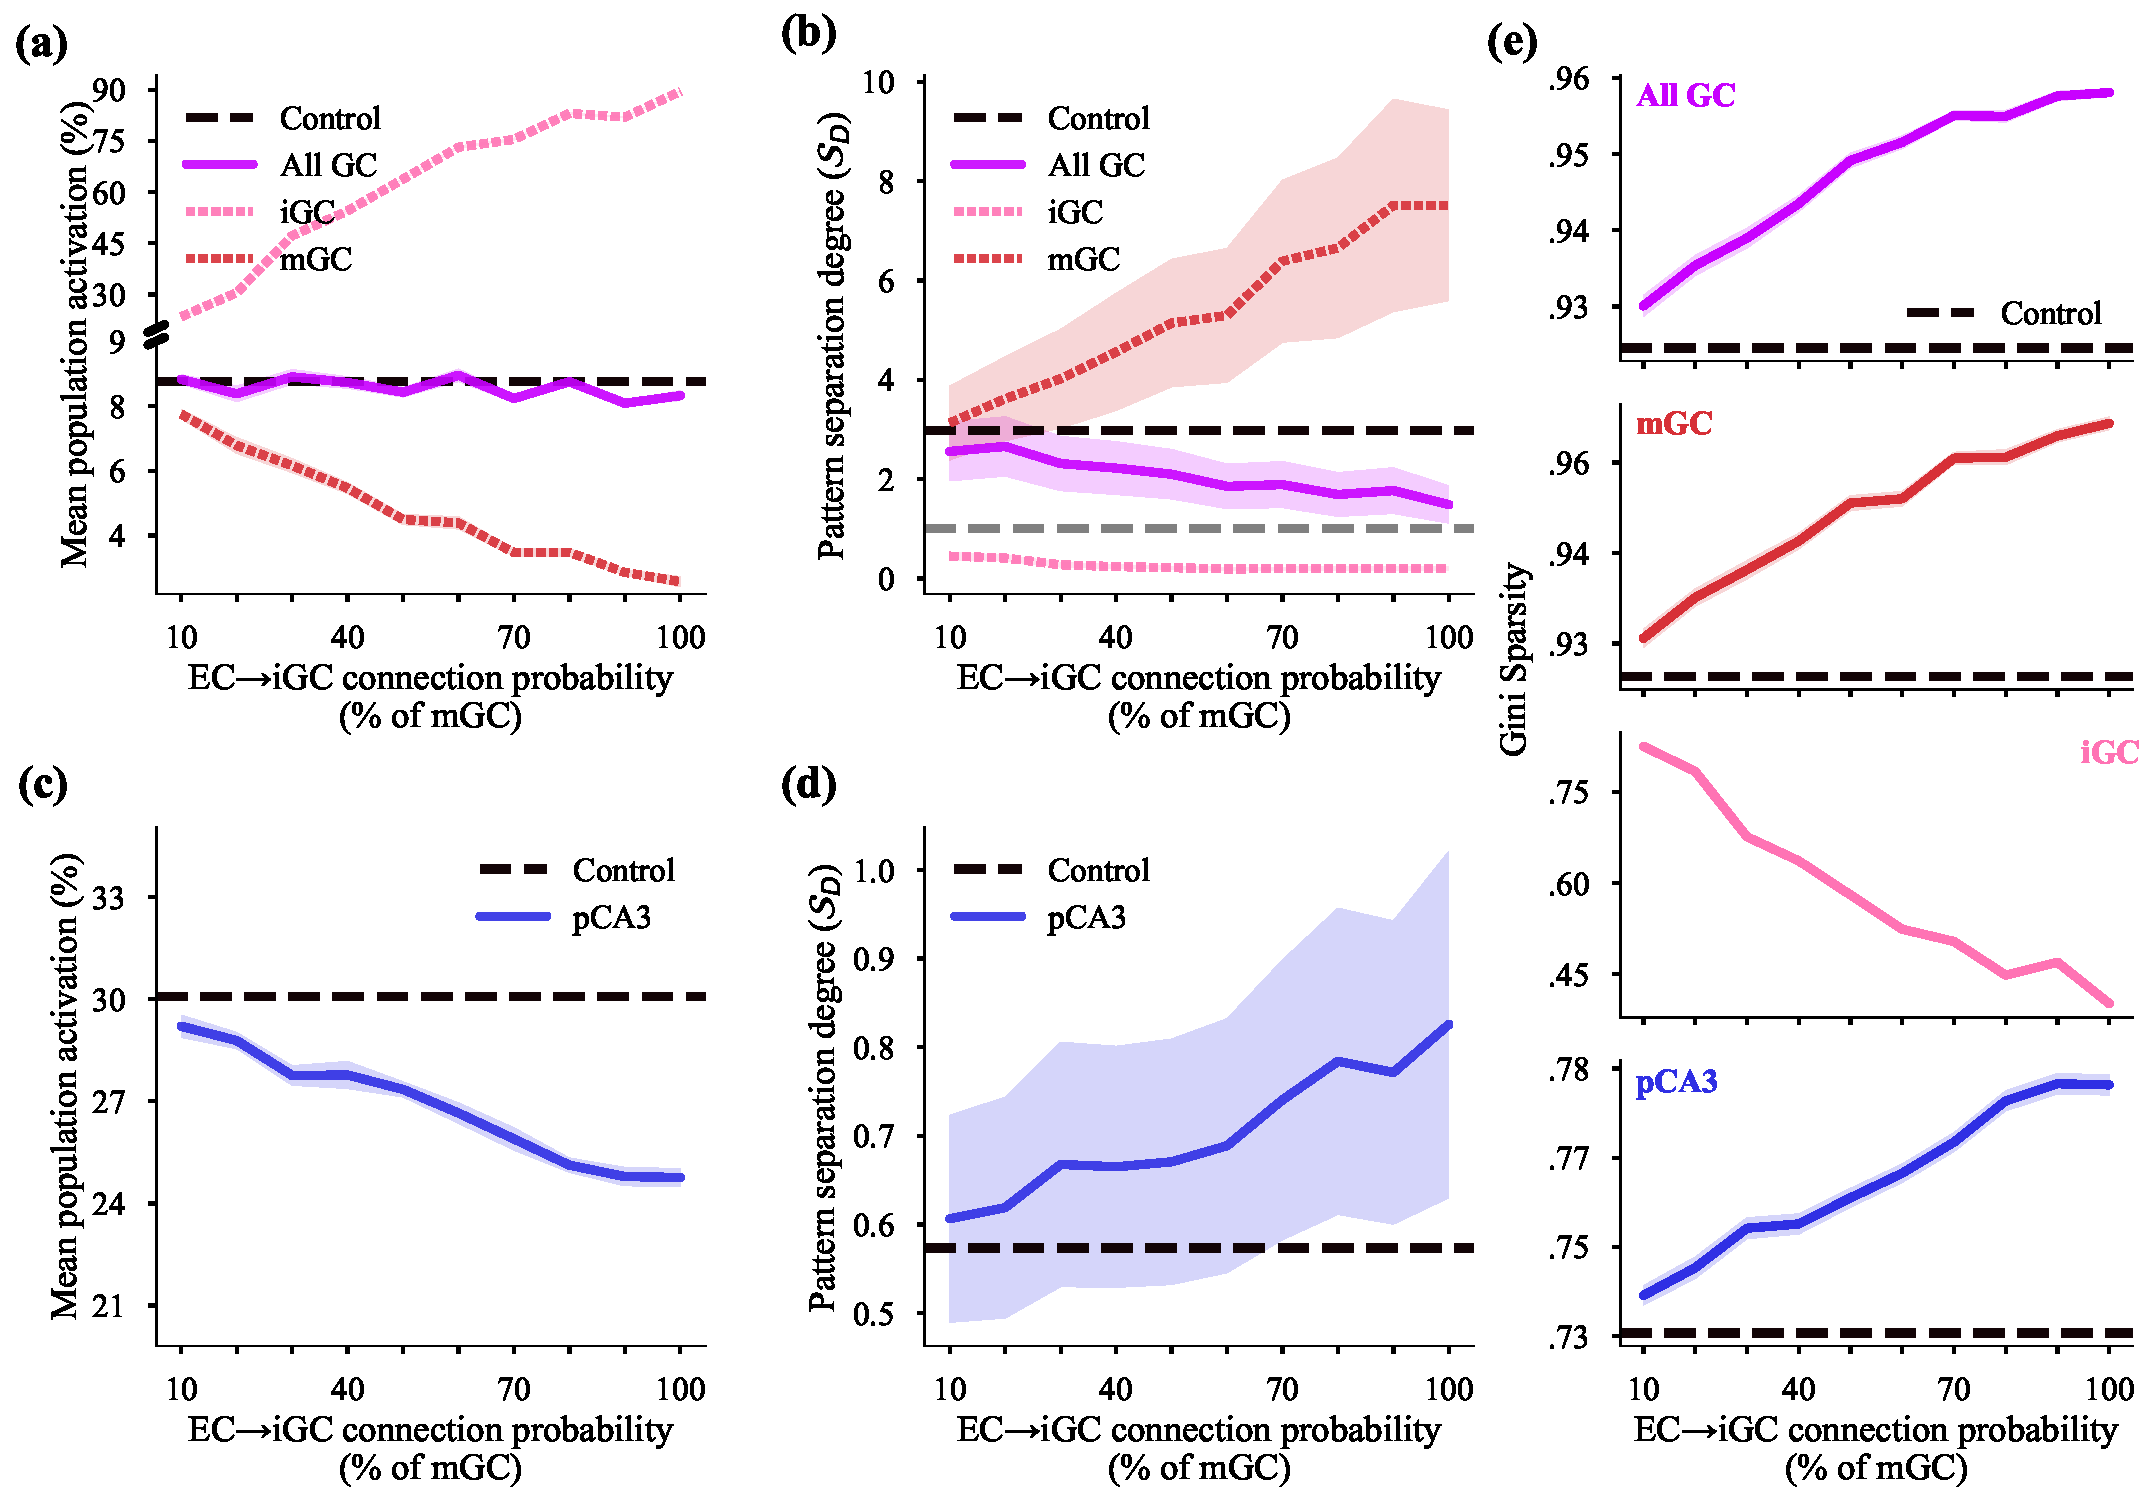
\includegraphics[width=\textwidth]{figures/plots/results_panel.pdf}%
\label{fig:results-2}
\end{figure}

\section{Enhanced separation is driven mainly by increased sparsity}\label{sec:res_sparsity}

Figure~\ref{fig:results-2}e shows that the sparsity indices of both the DG and the CA3 increase with neurogenesis and with the
increasing EC$\to$iGC connection probability, reproducing the central result of~\textcite{mchughAdultborn2022}, where adult-born
GCs promote population sparsity throughout the hippocampus. Across the ten connection probabilities, the Gini index rose
monotonically for the whole GC population (from $0.93$ to $0.96$; Spearman $\rho = +0.99$, $p < 10^{-6}$) and for the pCA3 cells
(from $0.74$ to $0.78$; $\rho = +0.99$, $p < 10^{-6}$), each above its control value. The Gini index is shown here; the Hoyer
measure, computed for cross-validation, follows the same trend (Figure~\ref{fig:sparsity_hoyer}).

The separation degree depends on both the orthogonalization degree and the activation degree of the patterns
(Equations~\ref{eq:dp}--\ref{eq:sd}), so the mGCs could separate better by making their outputs sparser, more decorrelated, or
both. Because the two combine multiplicatively, the change in $\log \mathcal{S}_D$ splits into an additive contribution from each.
Most of the increase (about 92\%) comes from the lower activation degree, as fewer mGCs fire for each pattern. The remaining 8\%
comes from a smaller but real gain in orthogonalization, as the mGC outputs become less correlated
(Figure~\ref{fig:mgc_orthogonalization}); this is not merely an effect
of the sparser activity, since it remains when the number of active cells is held fixed. This extra
decorrelation is likely due to the stronger winner-take-all competition driven by the iGCs~\parencite{coultripCortical1992}. The
entire GC population behaves the opposite: its decline in separation (Section~\ref{sec:res_separation}) stems almost entirely
(about 97\%) from the increased correlation among its outputs, rather than from any change in activation.

\section{iGC activation recruits circuit-wide inhibition}\label{sec:res_activation}

Directly injecting current into half of the iGCs propagated through the entire DG-CA3 network, as summarized by the PSTHs of
Figure~\ref{fig:psth}, pooled over all EC$\to$iGC connection probability variants.

Within the DG, the MCs were strongly excited and in turn drove strong excitation to the BCs. The BCs responded with a large,
significant increase in firing, organized as a synchronous population rhythm at $\sim\SI{127}{\hertz}$. The fast-spiking BCs are
able to sustain a rhythm of this frequency, as their firing rate reaches up to $\sim\SI{230}{\hertz}$ \textit{in
vivo}~\parencite{lubkeSpecialized1998}.

The HIPPs, by contrast, were only weakly inhibited (peak $z \approx -1$), a counterintuitive outcome given that they receive
excitatory input from both the iGCs and the MCs; a plausible cause is that the transient drop in overall GC output following the
pulse withdraws the GC$\to$HIPP excitation that would otherwise engage them, outweighing the direct MC drive.

The mGCs displayed a biphasic response to the activation of the iGCs: a small excitation at first (peak $z \approx 4$), followed
by an even smaller inhibition afterwards, with the net effect over the \SI{60}{\milli\second} being excitatory.

In CA3, the iCA3 interneurons were strongly and significantly activated, and this recruitment translated into a small inhibition
of the pCA3 cells through the iCA3$\to$pCA3 projection. \textcite{mchughAdultborn2022} reported this interneuron recruitment to
follow iGC spikes with a lag of \SIrange{20}{40}{\milli\second} \textit{in vivo}; because axonal conduction delays were not
modeled and all synaptic delays were fixed at \SI{1}{\milli\second}, the absolute latencies here are shorter and not directly
comparable, although the temporal ordering of the responses is preserved.

Comparing the Gini index of each population between the \SI{50}{\milli\second} windows immediately before and after the pulse
confirmed that this recruitment of inhibition increased population sparsity in most of the models, the within-trial counterpart of
the steady-state sparsification reported in Section~\ref{sec:res_sparsity}; the full comparison across populations and connection
probabilities is given in Figure~\ref{fig:opto_sparsity}. Overall, direct iGC activation recruited inhibitory interneurons across
both the DG and CA3.

\begin{figure}
    \centering
    \caption{Circuit-wide response to direct iGC activation. PSTHs of the population firing rate for each cell type, expressed as
        a z-score relative to a pre-pulse baseline (Equation~\ref{eq:psth_z}) and aligned to the onset of the
        \SI{5}{\milli\second} depolarizing current injected into half of the iGCs. The shaded band marks the pulse, in green for
        the directly stimulated iGCs and in gray for every other population. Bins are \SI{1.5}{\milli\second}
        wide and span \SIrange{-60}{60}{\milli\second} relative to the pulse; data are pooled over all EC$\to$iGC connection
        probability variants and all trials. Vertical scales differ across panels. The directly driven iGCs (top) dominate
        during the pulse; downstream, the MCs, BCs and iCA3 cells show strong excitation, the pCA3 cells and HIPPs a weaker
        inhibition, and the mGCs a small biphasic response.}

    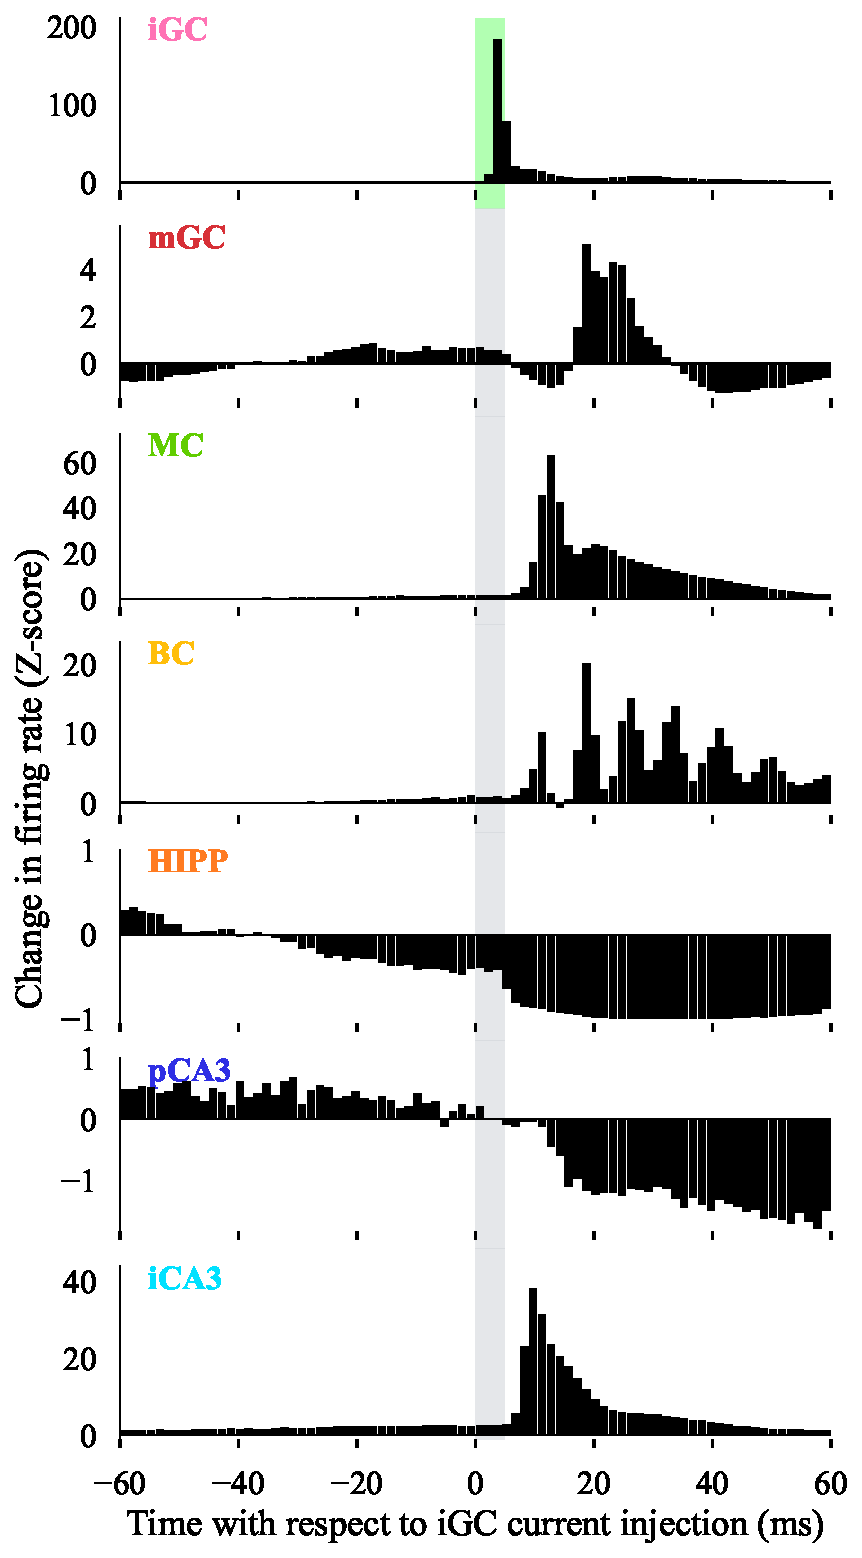
\includegraphics[width=0.65\textwidth]{figures/plots/psth_all.pdf}%
\label{fig:psth}
\end{figure}
